\documentclass[rnaas]{aastex62}

\pdfoutput=1

\usepackage{lmodern}
\usepackage{microtype}
\usepackage{url}
\usepackage{amsmath}
\usepackage{amssymb}
\usepackage{natbib}
\usepackage{multirow}
\usepackage{graphicx}
\bibliographystyle{aasjournal}

% ------------------ %
% end of AASTeX mods %
% ------------------ %

% Projects:
\newcommand{\project}[1]{\textsf{#1}}
\newcommand{\kepler}{\project{Kepler}}
\newcommand{\ktwo}{\project{K2}}

% references to text content
\newcommand{\documentname}{\textsl{Note}}
\newcommand{\figureref}[1]{\ref{fig:#1}}
\newcommand{\Figure}[1]{Figure~\figureref{#1}}
\newcommand{\figurelabel}[1]{\label{fig:#1}}
\renewcommand{\eqref}[1]{\ref{eq:#1}}
\newcommand{\Eq}[1]{Equation~(\eqref{#1})}
\newcommand{\eq}[1]{\Eq{#1}}
\newcommand{\eqalt}[1]{Equation~\eqref{#1}}
\newcommand{\eqlabel}[1]{\label{eq:#1}}

% TODOs
\newcommand{\todo}[3]{{\color{#2}\emph{#1}: #3}}
\newcommand{\dfmtodo}[1]{\todo{DFM}{red}{#1}}
\newcommand{\alltodo}[1]{\todo{TEAM}{red}{#1}}
\newcommand{\citeme}{{\color{red}(citation needed)}}

% math
\newcommand{\T}{\ensuremath{\mathrm{T}}}
\newcommand{\dd}{\ensuremath{ \mathrm{d}}}
\newcommand{\unit}[1]{{\ensuremath{ \mathrm{#1}}}}
\newcommand{\bvec}[1]{{\ensuremath{\boldsymbol{#1}}}}
\newcommand{\Gaussian}[3]{\ensuremath{\frac{1}{|2\pi #2|^\frac{1}{2}}
            \exp\left[ -\frac{1}{2}#1^\top #2^{-1} #1 \right]}}

% VECTORS AND MATRICES USED IN THIS PAPER
\newcommand{\Normal}{\ensuremath{\mathcal{N}}}
\newcommand{\mA}{\ensuremath{\bvec{A}}}
\newcommand{\mC}{\ensuremath{\bvec{C}}}
\newcommand{\mS}{\ensuremath{\bvec{\Sigma}}}
\newcommand{\mL}{\ensuremath{\bvec{\Lambda}}}
\newcommand{\vw}{\ensuremath{\bvec{w}}}
\newcommand{\vy}{\ensuremath{\bvec{y}}}
\newcommand{\vt}{\ensuremath{\bvec{\theta}}}
\newcommand{\vm}{\ensuremath{\bvec{\mu}(\bvec{\theta})}}
\newcommand{\vre}{\ensuremath{\bvec{r}}}
\newcommand{\vh}{\ensuremath{\bvec{h}}}
\newcommand{\vk}{\ensuremath{\bvec{k}}}

% typography obsessions
\setlength{\parindent}{3.0ex}

\begin{document}\raggedbottom\sloppy\sloppypar\frenchspacing

\title{%
Robust moment maps for ALMA observations
}

\author[0000-0003-1534-5186]{Richard Teague}
\affil{University of Michigan, Ann Arbor, MI}

\author[0000-0002-9328-5652]{Daniel Foreman-Mackey}
\affil{Flatiron Institute, New York, NY}

%\keywords{%
%methods: data analysis ---
%methods: statistical
%}

\section{Introduction}

Inferring the line of sight velocity from Doppler shifted spectra is a commonly used analysis in the study of protoplanetary disks, galaxies and star forming regions. Multiple approaches in collapsing a data cube to a single velocity at each pixel exist in the literature \citep[see, for example][]{deBlok:2008}, however the two most common approaches are `first moment maps' or the velocity of the maximum intensity, called the `ninth moment' when calculated using \texttt{CASA} (although a minomer as it does not relate to a statistical moment, we adopt this terminology for this note).

The first moment approach is strongly affected by the noise in the spectrum and the (a)symmetry of the intrinsic profile. Clipping the data below some signal-to-noise value or masking the data are typically used to avoid these issues, placing a strong prior on the emission distribution, potentially introducing (or removing) features in the data. These issues can be avoided using the velocity of the maximum pixel, however the precision of this approach is limited by the velocity resolution of the data.

Other approaches involve fitting a line profile believed to be representative of the true line profile. In addition to be computationally expensive, this approach implicitly assumes that the true line profile is known, but deviations from this profile can often lead to incorrect inferences. For example, spatially resolved protoplanetary disks have been be shown to have a two-Gaussian component as emission is observed from both the front side of the disk as well as the rear \citep{Rosenfeld:2013} and the fitting of a single Gaussian component will bias the result.

In this research note we demonstrate a new method to infer the line-of-sight velocity component which combines the sub-channel precision from the first moment map method and the model independence of the ninth moment approach.

\section{Technical details}

It has been demonstrated that fitting a quadratic surface to astronomical
imaging can produce near-optimal estimates of source centroids
\citep{Vakili:2016}.
Here we apply this method to estimate the velocity centroid in each pixel
non-parametrically.
This method has the benefit of being less sensitive to the shape of the wings
of the line spread function than standard moment estimation methods.
Unlike the `ninth moment' method, our quadratic method achieves sub-pixel
precision in the velocity estimates.

The fundamental idea upon which this method is built is that we can fit a
quadratic model to the intensity values surrounding the maximum pixel and
analytically maximize that function to find the velocity estimate.
Following \citet{Vakili:2016}, we find the pixel of maximum intensity in the
spectrum and extract that pixel value $f_0$ and the one to the left $f_-$ and
right $f_+$.
Modeling these three intensities as a quadratic
\begin{eqnarray}
f(x) &=& a_0 + a_1\,(x-x_0) + a_2\,{(x-x_0)}^2
\eqlabel{quad}
\end{eqnarray}
where $x_0$ is the pixel coordinate of maximum intensity and $x$ is in units
of pixels, we find
\begin{eqnarray}
a_0 &=& f_0 \\
a_1 &=& \frac{1}{2}(f_+ - f_-) \\
a_2 &=& \frac{1}{2}(f_+ + f_- - 2\,f_0) \quad.
\end{eqnarray}
By maximizing \Eq{quad}, we find the following estimate for the pixel
coordinate of maximum velocity:
\begin{eqnarray}
x_\mathrm{max} &=& x_0 - \frac{a_1}{2\,a_2} \\
    &=& x_0 - \frac{f_+ - f_-}{2\,(f_+ + f_- - 2\,f_0)} \quad.
\end{eqnarray}

We can also estimate the statistical uncertainty on $x_\mathrm{max}$ by
propagating the uncertainty from the fluxes to uncertainties on the polynomial
coefficients.
If we assume independent Gaussian uncertainties on the fluxes with standard
deviation $\sigma$, the covariance matrix for the polynomial coefficients
$\bvec{a} = {(a_2,\,a_1,\,a_0)}^\T$ is
\begin{eqnarray}
\Sigma_\bvec{a} = \sigma^2\,\left(\begin{array}{ccc}
\frac{3}{2} \quad & \quad 0 \quad &\quad 1 \\
0\quad &\quad \frac{1}{2}\quad &\quad 0 \\
-1\quad &\quad 0\quad &\quad 1
\end{array}\right)\quad.
\end{eqnarray}
Using these values and linearized propagation of uncertainty, we find the
following approximation for the \emph{statistical} uncertainty on
$x_\mathrm{max}$
\begin{eqnarray}
{\sigma_{x_\mathrm{max}}}^2 = \frac{\sigma^2}{8}\,\left[
    \frac{3}{{a_2}^2} + \frac{{a_1}^2}{{a_2}^4}
\right]\quad.
\end{eqnarray}
We emphasize that there are other sources of systematic uncertainty that must
be considered in production.

\section{Demonstration of Method}

\begin{figure}[htbp]
\centering
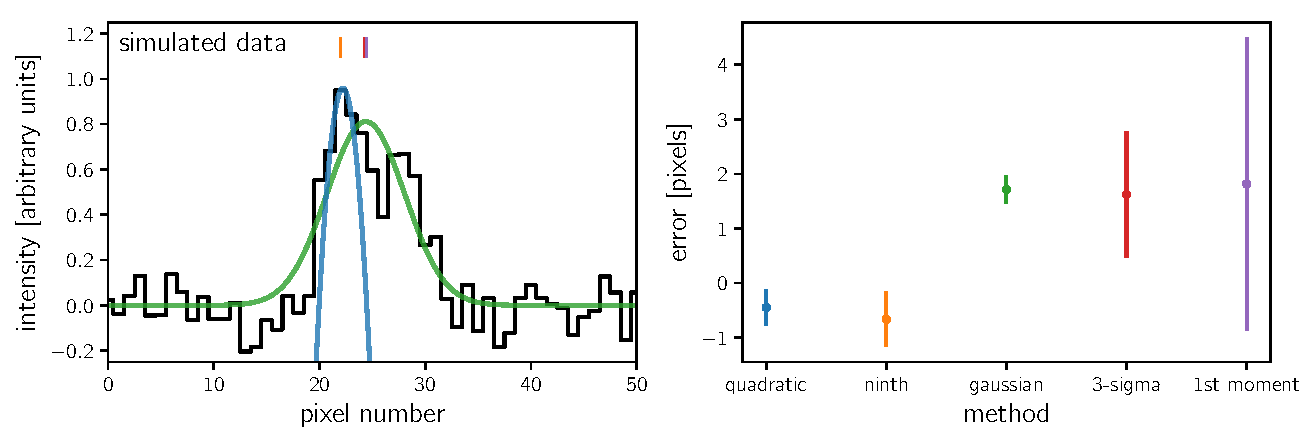
\includegraphics[width=\textwidth]{../notebooks/simulated-spectrum.pdf}
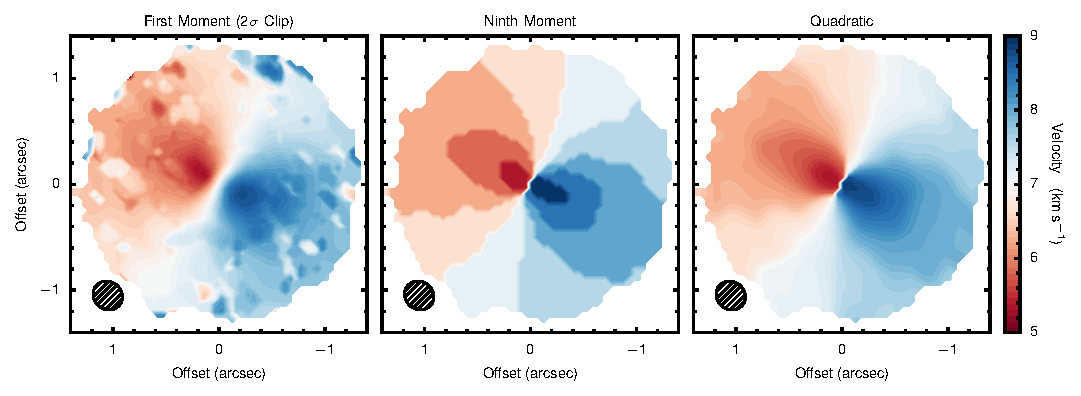
\includegraphics{moment_comparison.pdf}
\caption{Top row: Comparisons of methods used to infer the velocity profile and their associated accuracy and precision. Bottom row: comparisons of methods used to infer the velocity of HD~135344B. \label{figure}}
\end{figure}

The top row of Fig.~\ref{figure} compares the accuracy and precision of different approaches for a non-Gaussian line profile. The left panel shows in blue the quadratic fit to the peak pixel and the neighboring pixels, while in green shows a Gaussian profile fit. The orange, red and purple vertical lines show the inferred velocity using the ninth moment method and the first moment method with both a $3\sigma$ clip and no clipping, respectively. The right hand panel compares the accuracy and precision of these methods.

As a demonstration with real data, we image Atacama Large (sub-)Millimeter Array observations of $^{13}$CO in the well studied protoplanetary disk HD~135344B at a velocity resolution of $330~{\rm m\,s^{-1}}$ \citep[ALMA Project 2012.1.00158.S]{vanderMarel:2016} . The bottom row of Fig.~\ref{figure} compares the inferred line-of-sight velocity using, left to right, the intensity weighted average (first moment map), clipping all values below $3\sigma$, the velocity of the maximum intensity, and finally the quadratic approach described in the previous section. Clearly the first moment approach suffers from noise features which are dependent on the level of clipping applied. The ninth moment is not affected by such features, however is limited in precision by the observations. The quadratic approach does not suffer from noise features while maintaining a high precision on the inferred velocity.

\bibliography{bettermoments}



\end{document}
